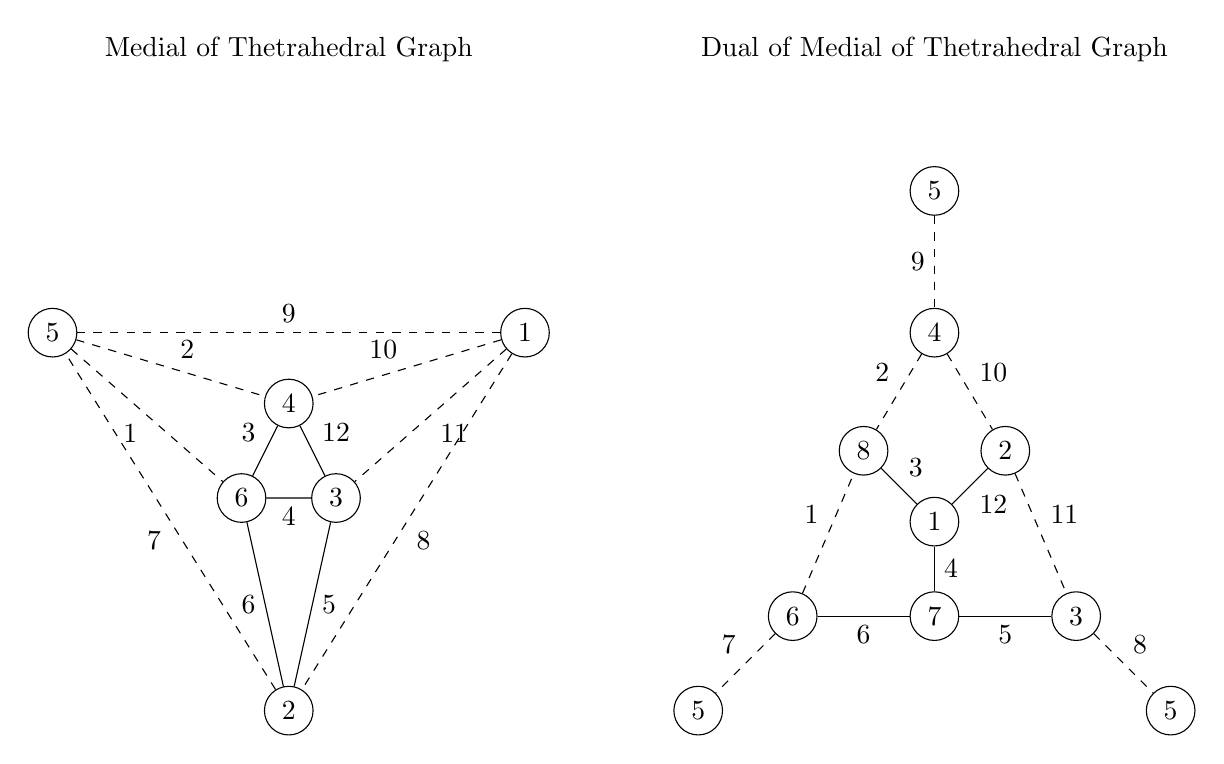
\begin{tikzpicture}
	% Define the nodes with specific positions
	\begin{scope}[xshift=0cm, yshift=0cm, scale=0.6]
		\node (G) at (3, 6) {Medial of Thetrahedral Graph};

		\node[circle, draw] (1) at (8, -0) {1};
		\node[circle, draw] (2) at (3, -8) {2};
		\node[circle, draw] (3) at (4, -3.5) {3};
		\node[circle, draw] (4) at (3, -1.5) {4};
		\node[circle, draw] (5) at (-2, -0) {5};
		\node[circle, draw] (6) at (2, -3.5) {6};
	
		% Draw the edges between nodes with labels
		\draw[dashed] (5) -- node[below left] {1} (6);
		\draw[dashed] (5) -- node[above right] {2} (4);
		\draw[draw] (4) -- node[above left] {3} (6);
		\draw[draw] (3) -- node[below] {4} (6);
		\draw[draw] (3) -- node[right] {5} (2);
		\draw[draw] (6) -- node[left] {6} (2);
		\draw[dashed] (2) -- node[below left] {7} (5);
		\draw[dashed] (1) -- node[below right] {8} (2);
		\draw[dashed] (1) -- node[above] {9} (5);
		\draw[dashed] (1) -- node[above left] {10} (4);
		\draw[dashed] (1) -- node[below right] {11} (3);
		\draw[draw] (4) -- node[above right] {12} (3);
	\end{scope}

	\begin{scope}[xshift=10cm, yshift=-2.4cm, scale=0.6]
		\node (G) at (0, 10) {Dual of Medial of Thetrahedral Graph};

		\node[circle, draw] (d1) at (0, 0) {1};
		\node[circle, draw] (d2) at (1.5, 1.5) {2};
		\node[circle, draw] (d3) at (3, -2) {3};
		\node[circle, draw] (d4) at (0, 4) {4};
		\node[circle, draw] (d51) at (0, 7) {5};
		\node[circle, draw] (d52) at (5, -4) {5};
		\node[circle, draw] (d53) at (-5, -4) {5};
		\node[circle, draw] (d6) at (-3, -2) {6};
		\node[circle, draw] (d7) at (0, -2) {7};
		\node[circle, draw] (d8) at (-1.5, 1.5) {8};
	
		% Draw the edges between nodes with labels
		\draw[dashed] (d6) -- node[above left] {1} (d8);
		\draw[dashed] (d4) -- node[above left] {2} (d8);
		\draw[draw] (d1) -- node[above right] {3} (d8);
		\draw[draw] (d7) -- node[right] {4} (d1);
		\draw[draw] (d7) -- node[below] {5} (d3);
		\draw[draw] (d6) -- node[below] {6} (d7);
		\draw[dashed] (d6) -- node[above left] {7} (d53);
		\draw[dashed] (d3) -- node[above right] {8} (d52);
		\draw[dashed] (d51) -- node[left] {9} (d4);
		\draw[dashed] (d4) -- node[above right] {10} (d2);
		\draw[dashed] (d2) -- node[above right] {11} (d3);
		\draw[draw] (d1) -- node[below right] {12} (d2);
	\end{scope}
\end{tikzpicture}